% Kyle: TODO: stratified grape example: better
\section{ Spatial sampling }
% Show the reason that indices are likely to converge to a set of locations over and over again...
The current spatial sampling method simply focuses on iteratively moving points to locations that are far away from all other points. <List the iterative scoring method to maximize>
% show no real increase in performance for apple datasets
\begin{figure}
\centering
\parbox{7cm}
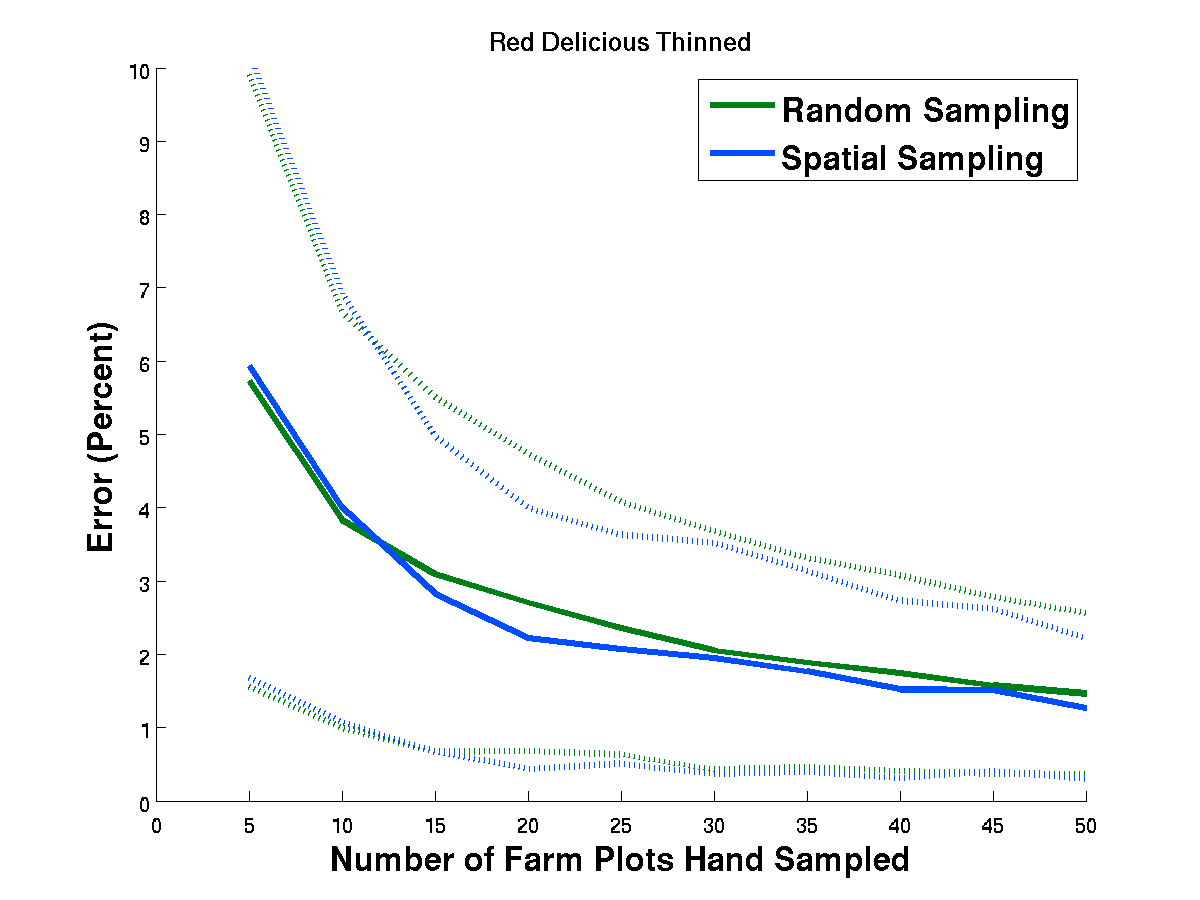
\includegraphics[width=5cm]{apple/Red_Delicious/Red_Delicious_Thinned_Spatial_Sampling.png}
\caption{Red Delicious}
\label{fig:Red_Delicious_Thinned_Spatial_Sampling}
\qquad
\begin{minipage}{7cm}
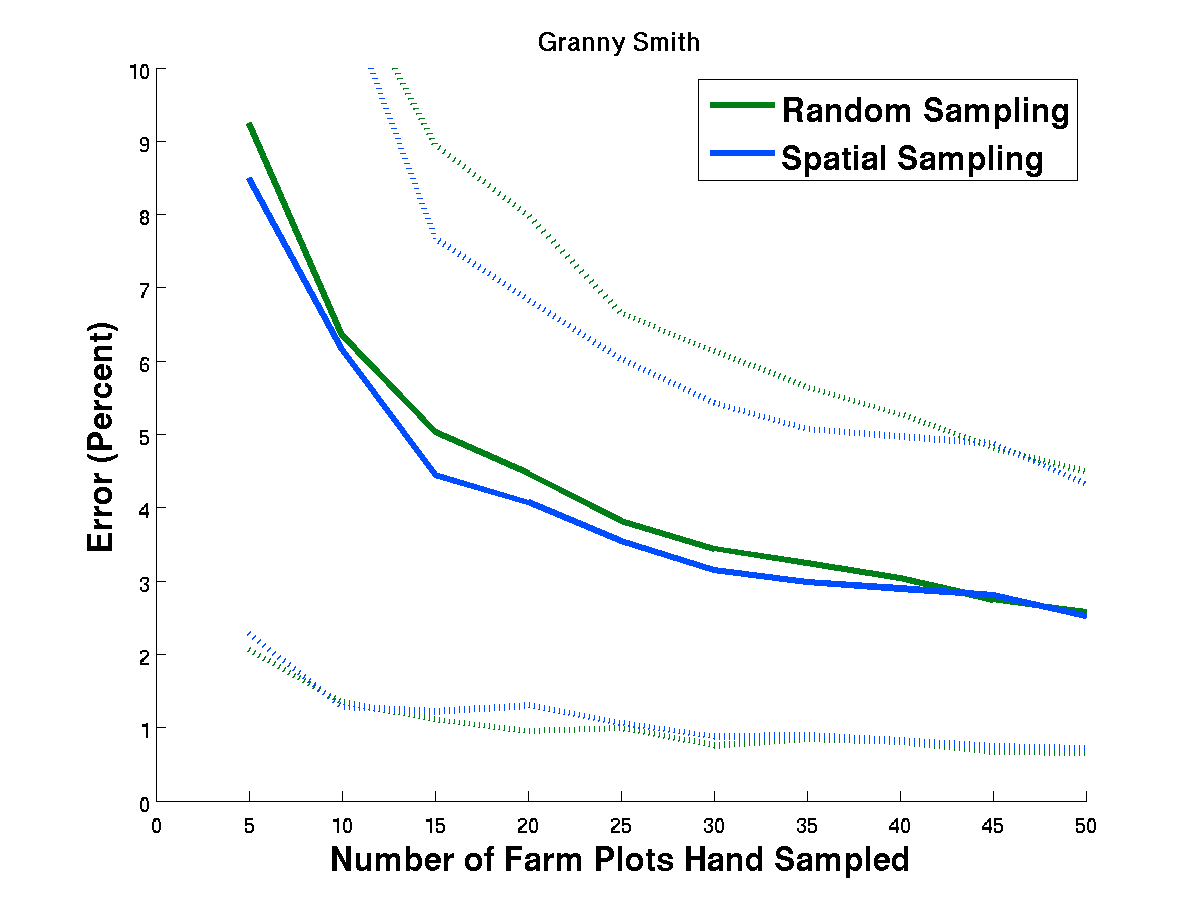
\includegraphics[width=5cm]{apple/Granny_Smith/Granny_Smith_Spatial_Sampling.png}
\caption{Granny Smith}
\label{fig:Granny_Smith_Spatial_Sampling}
\end{minipage}
\end{figure}

\section{Results}
\subsection{ Sampling: Scaling with a scalar value }
% show spatial and stratified
% for all of the grape datasets

\subsection{ Direct Extrapolation: No Sensor Data }
All of our sampling methods are based on a process that starts with initially sampling groundtruth data. In this section, the results show that simply extrapolating this groundtruth subsample measurement can gain accuracy that is greater than scaling the sensor data.

% apple
For the apple datasets, it is seen that adding sensor data does in fact add accuracy. This is seen for both Granny Smith and Red Delicious apple datasets.
\begin{figure}
\centering
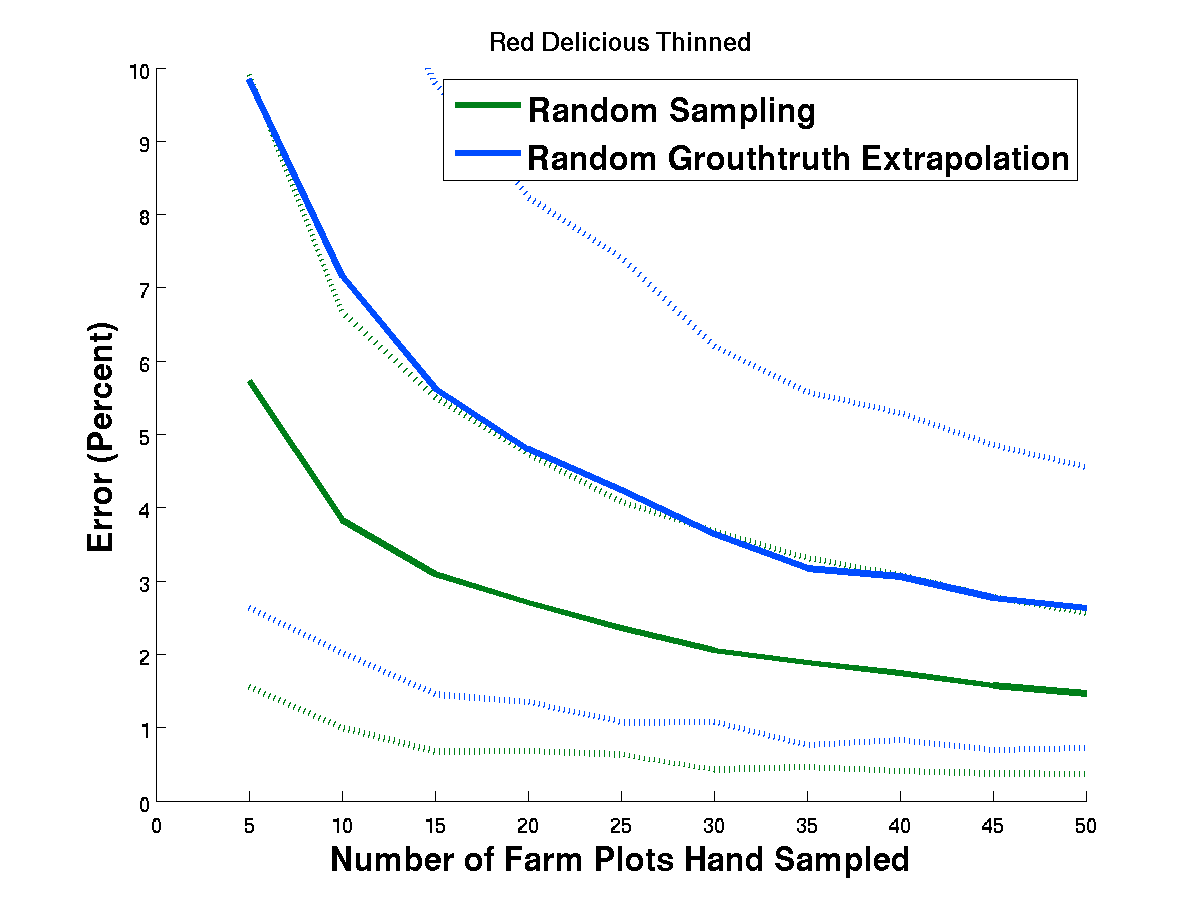
\includegraphics[width=0.8\linewidth]{apple/Red_Delicious/Red_Delicious_Thinned_Random_Grouthtruth_Extrapolation.png}
\caption{Red Delicious}
\label{fig:Red_Delicious_Thinned_Random_Grouthtruth_Extrapolation}
\end{figure}

% grape
For the grape datasets, direct extrapolation of the groundtruth is more effective than using sensor data. It is worth remembering that the sensor data would still provide dense image measurements that would be lost with a direct groundtruth extrapolation approach.
\begin{figure}
\centering
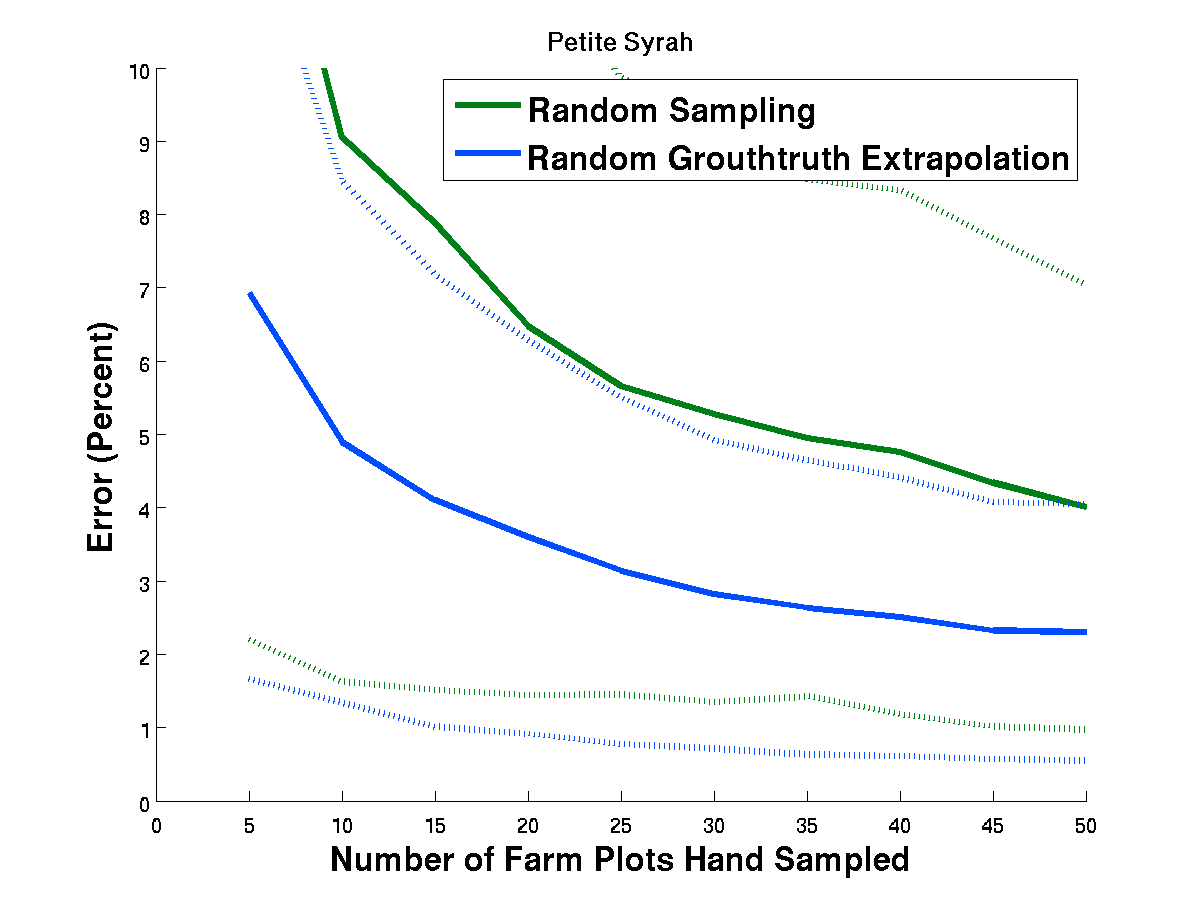
\includegraphics[width=0.8\linewidth]{grape/PS/Petite_Syrah_Random_Grouthtruth_Extrapolation.png}
\caption{Petite Syrah Groundtruth Extrapolation}
\label{fig:Petite_Syrah_Random_Grouthtruth_Extrapolation}
\end{figure}

This phenomenon is explained by the linear offset apparent in grape datasets described in the next section.

\subsection{ Sampling: Scaling with a linear function }
Instead of scaling with a scalar value, a linear scaling function can be obtained by doing linear regression on the subsample data collected. With this function, sensor data can be mapped to predicted yield in a more dynamic way.

% example of better performance
% grape
A linear function is seen to be effective for grape datasets.

\begin{figure}
\centering
\parbox{7cm}
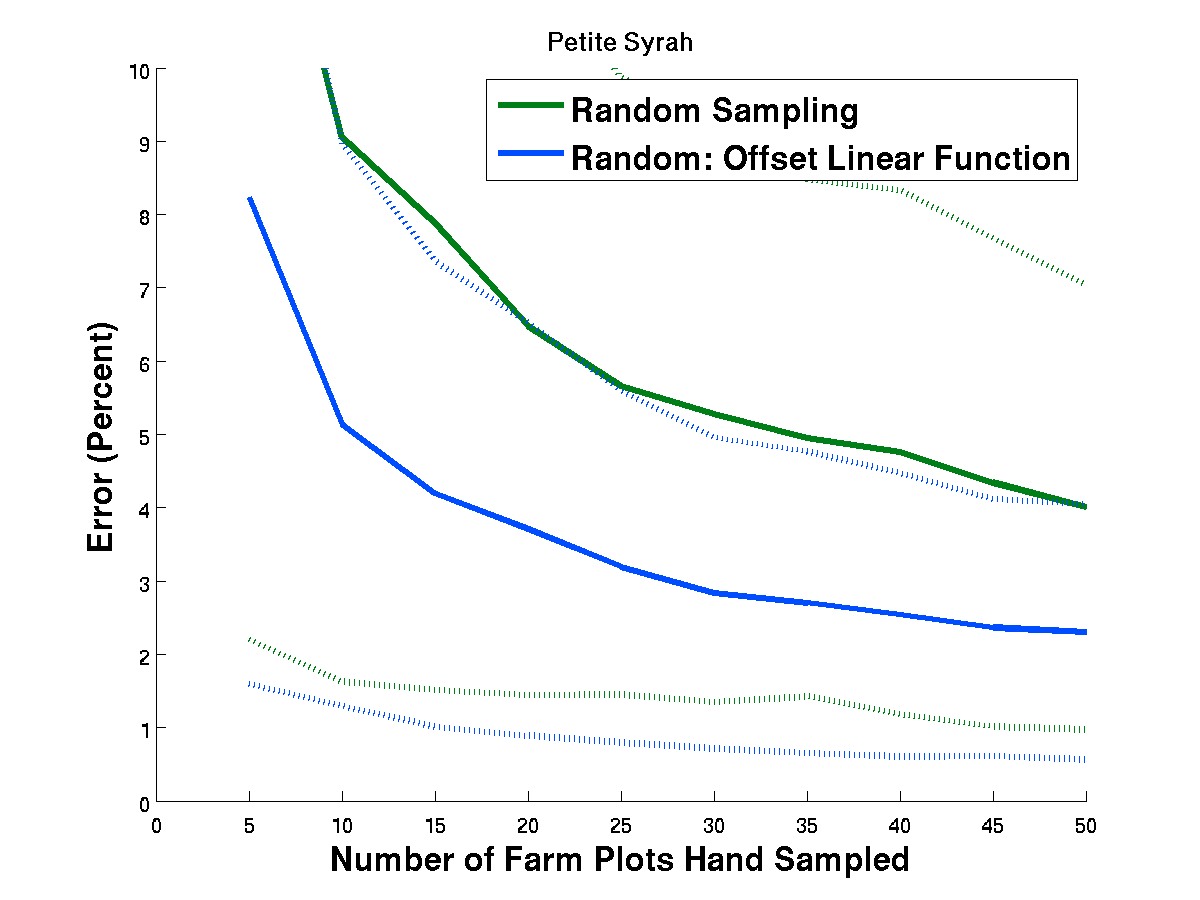
\includegraphics[width=0.8\linewidth]{grape/PS/Petite_Syrah_Random:_Offset_Linear_Function.png}
\caption{Petite Syrah}
\label{fig:Petite_Syrah_Random:_Offset_Linear_Function}
\qquad
\begin{minipage}{7cm}
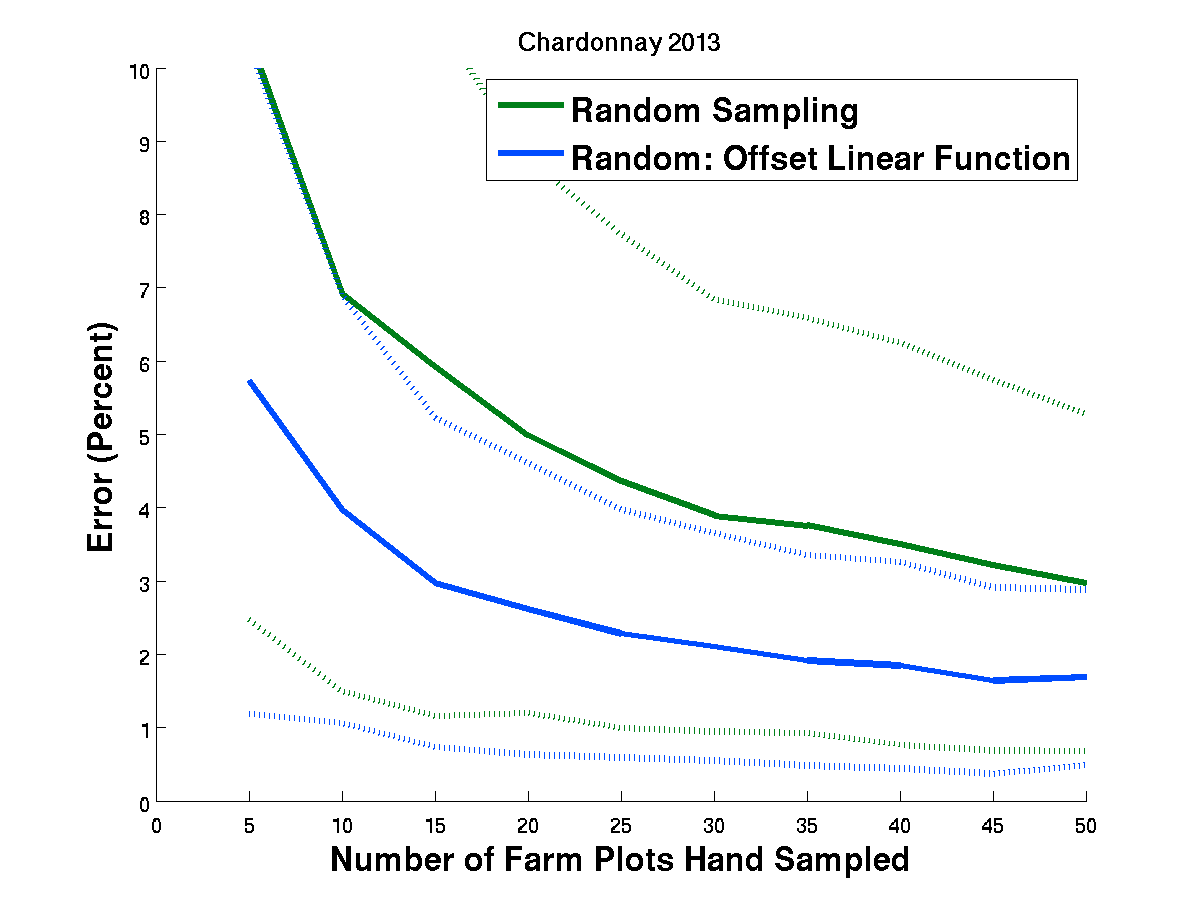
\includegraphics[width=0.8\linewidth]{grape/Chardonnay_2013/Chardonnay_2013_Random:_Offset_Linear_Function.png}
\caption{Chardonnay}
\label{fig:Chardonnay_2013_Random:_Offset_Linear_Function}
\end{minipage}
\end{figure}

% example of no improvement
% apple
A linear function is seen to be ineffective for apple datasets.
\begin{figure}
\centering
\parbox{7cm}
\includegraphics[width=5cm]{apple/Red_Delicious/Red_Delicious_Random:_Offset_Linear_Function.png}
\caption{Red Delicious}
\label{fig:Red_Delicious_Random:_Offset_Linear_Function}
\qquad
\begin{minipage}{7cm}
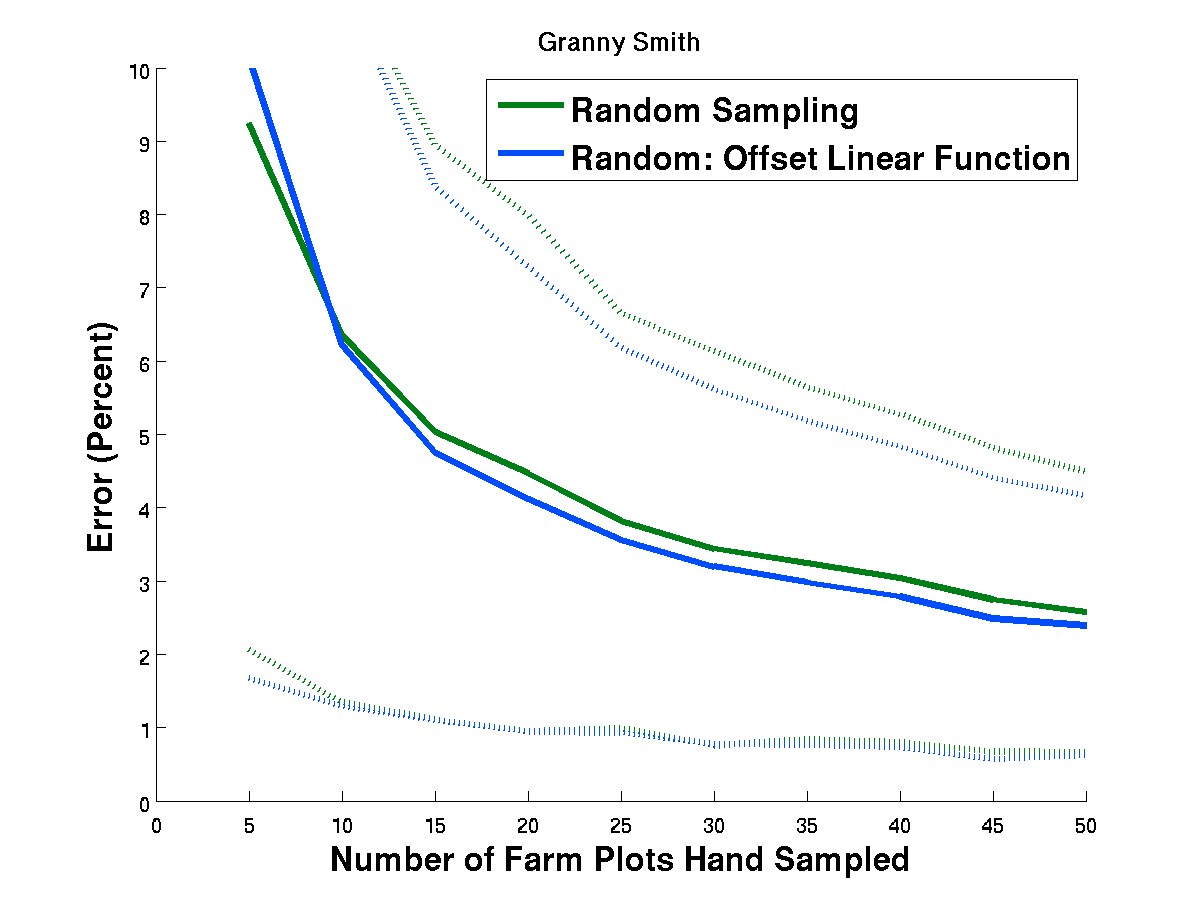
\includegraphics[width=5cm]{apple/Granny_Smith/Granny_Smith_Random:_Offset_Linear_Function.png}
\caption{Granny Smith}
\label{fig:Granny_Smith_Random:_Offset_Linear_Function}
\end{minipage}
\end{figure}

This suggests that there are some systematic differences between apple detection and grape detection. This is logical as the grape code includes features that the apple code does not, such as initial detection clustering.

\section{ Conclusion }
This document summarizes results found between July and August 2014, with regards to sampling methods in orchards and vineyards. This includes an analysis of sampling methods that revolve around a scaling factor: random, stratified random, and spatial. In addition, this also includes an analysis of pure groundtruth extrapolation and the usage of a linear function instead of a scaling factor.

The main takeaway conclusion from these results is different for apple and grape datasets.

For grape datasets, stratified and spatial sampling approaches does not improve performance. In fact, both led to a decrease in performance. Improvements, instead came from either using a linear function for scaling sensor data or directly extrapolating sensor data. In fact, directly extrapolating the groundtruth subsample yields similar accuracy as using a linear scaling function and any sampling method (stratified, spatial, random) for all 3 datasets. The message from these results is that 1.) a linear scaling function is necessary and 2.) the sensor data is not adding much signal currently.

For apple datasets, stratified and spatial sampling lead to small increases in performance that are marginal. A linear scaling function or direct extrapolation of groundtruth measurements did not lead to performance increases.

